\section{Модель исходной информационной системы}

Контекстная диаграмма исходной модели информационной системы представлена на рисунке~\ref{img:source-context}.

\begin{figure}[h!]
	\begin{center}
		\begin{minipage}[h]{\linewidth}
			\centering
			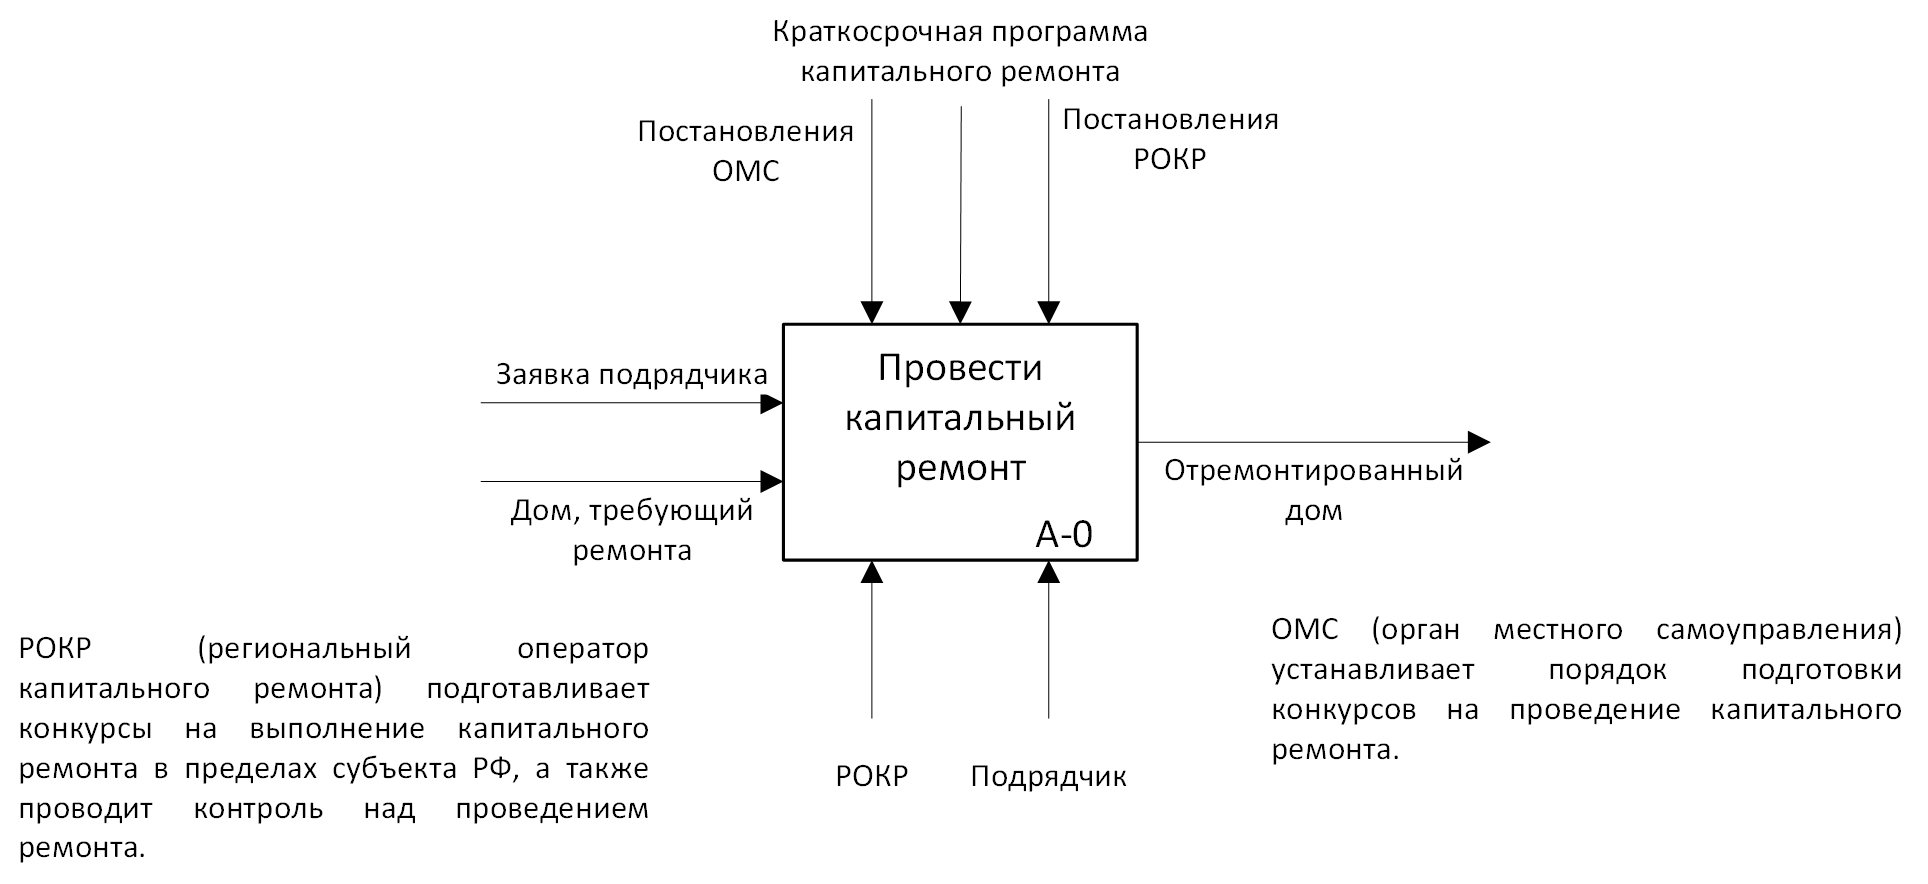
\includegraphics[width=\linewidth]{images/source-context.png}
			\caption{Контекстная диаграмма исходной модели}
			\label{img:source-context}
		\end{minipage}
		\hfill
	\end{center}
\end{figure}

Как можно заметить, для проведения капитального ремонта требуется наличие долгосрочной программы КР.
Существует две роли, выполняющий обязательства -- региональный оператор капитального ремонта и подрядная организация.
Процесс капитального ремонта происходит при регулировании постановлениями органов местного самоуправления, а также постановлениями РОКР.
Результатом капитального ремонта является его проведение.

Декомпозиция контекстной диаграммы представлена на рисунке~\ref{img:source-A0}.

\begin{figure}[h!]
	\begin{center}
		\begin{minipage}[h]{\linewidth}
			\centering
			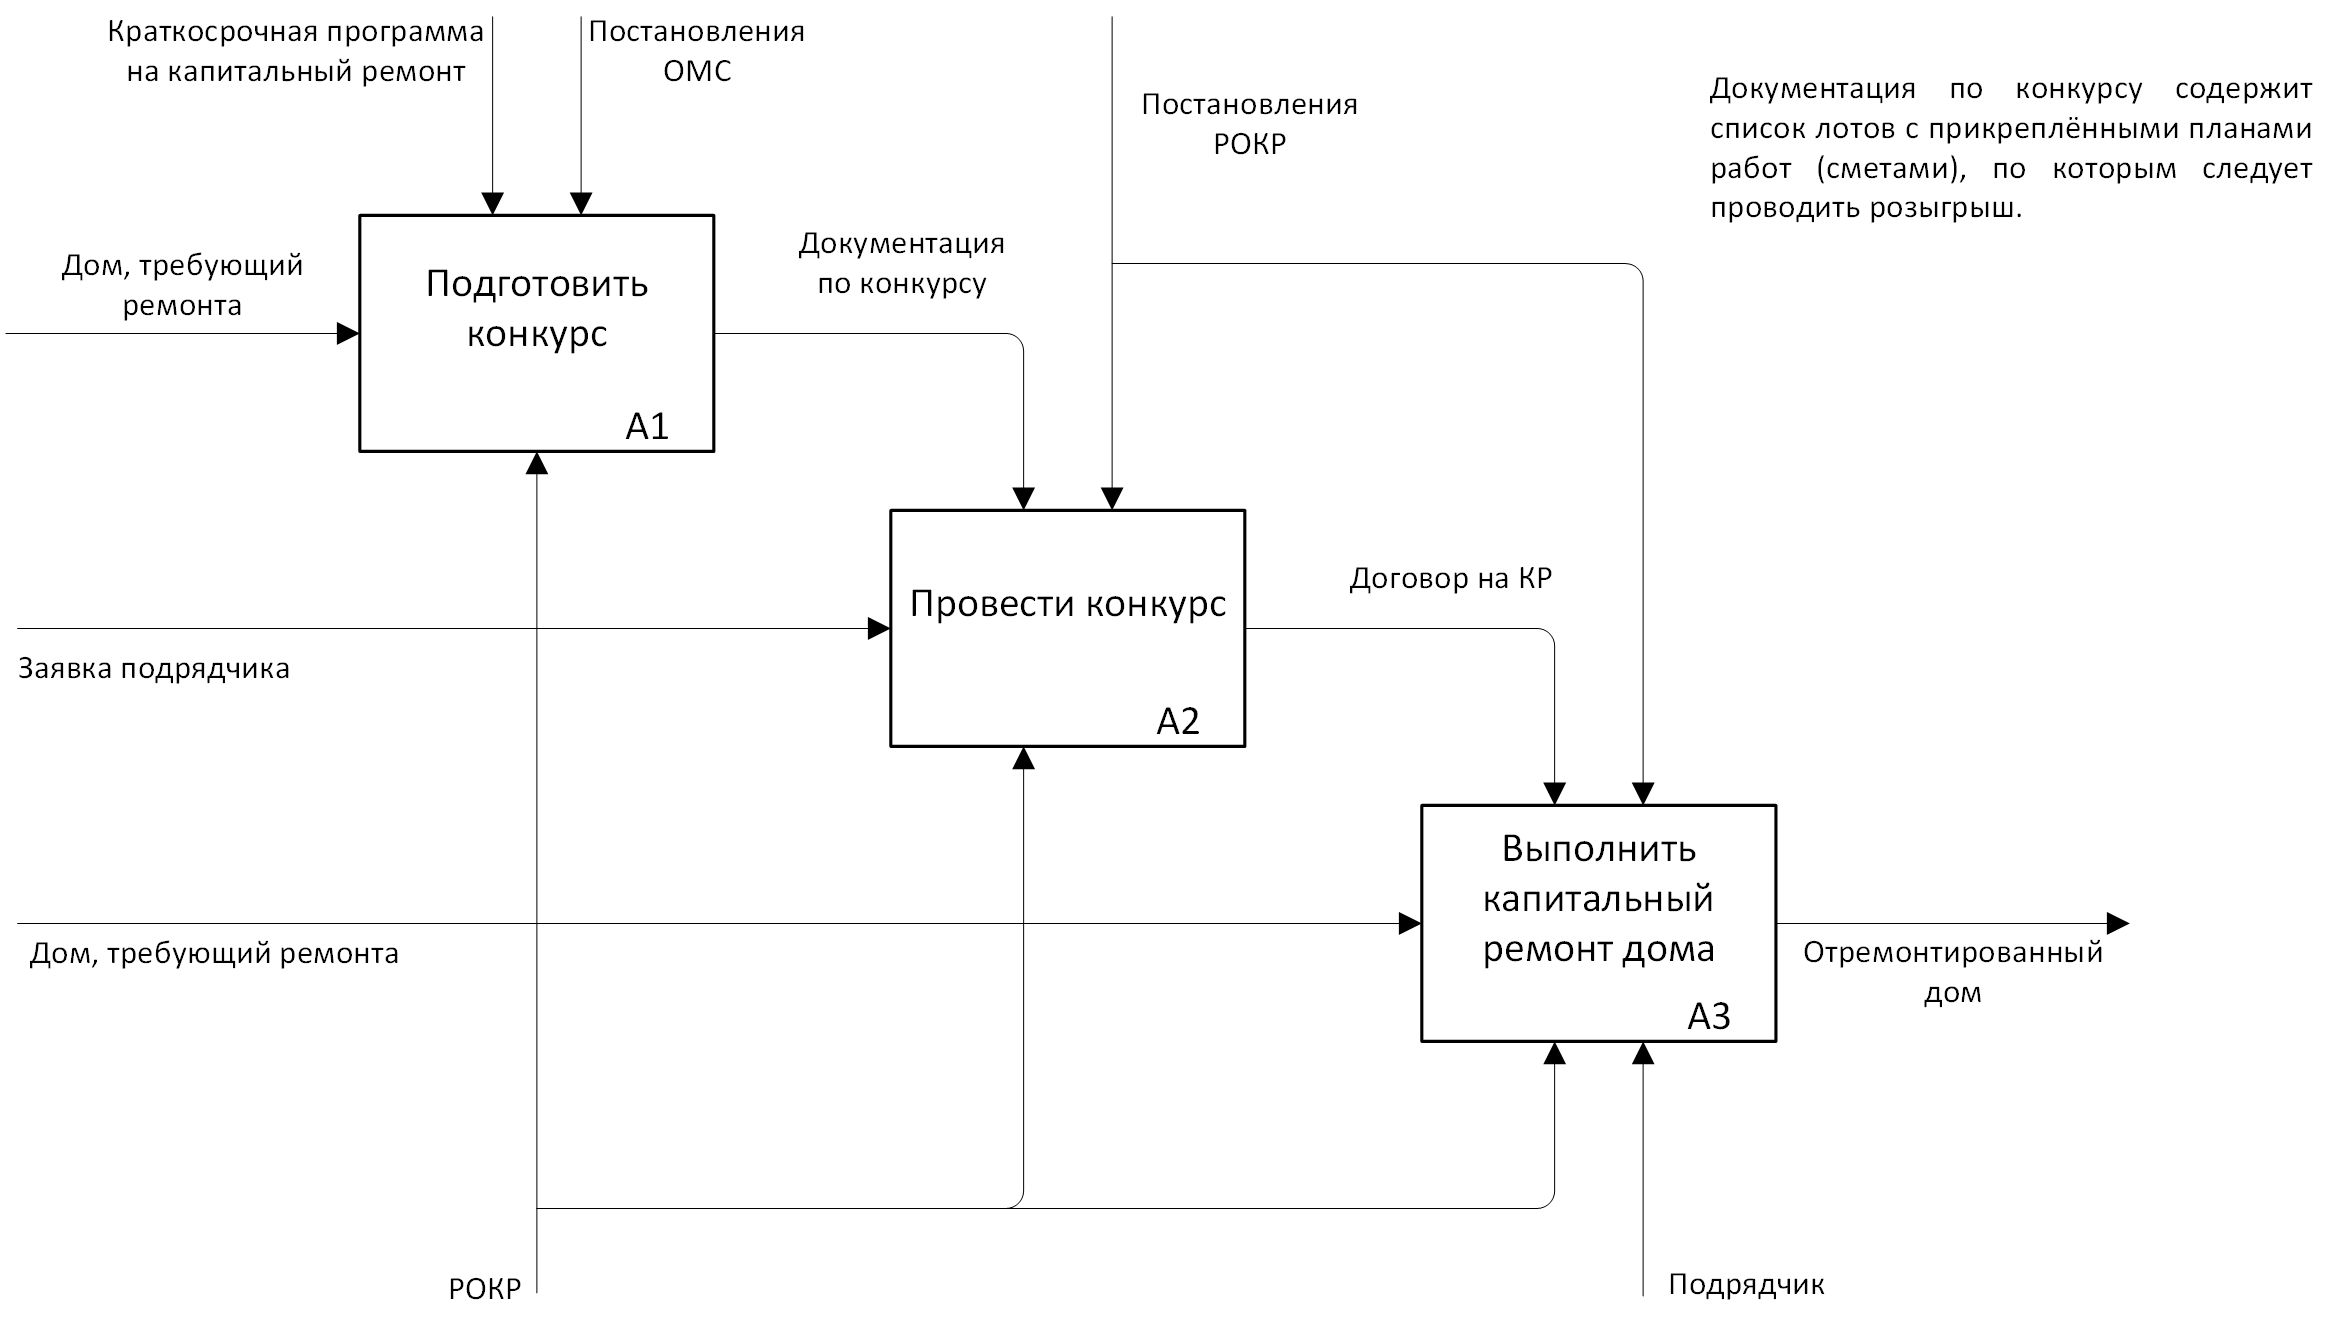
\includegraphics[width=\linewidth]{images/source-A0.png}
			\caption{Декомпозиция контекстной диаграммы}
			\label{img:source-A0}
		\end{minipage}
		\hfill
	\end{center}
\end{figure}

Процесс капитального ремонта состоит из трёх подпроцессов:

\begin{enumerate}
	\item формирование конкурсов на капитальный ремонт;
	\item проведение конкурсов на капитальный ремонт;
	\item собственно капитальный ремонт жилого фонда.
\end{enumerate}

Декомпозиция формирования конкурсов представлена на рисунке~\ref{img:source-A1}.

\begin{figure}[h!]
	\begin{center}
		\begin{minipage}[h]{\linewidth}
			\centering
			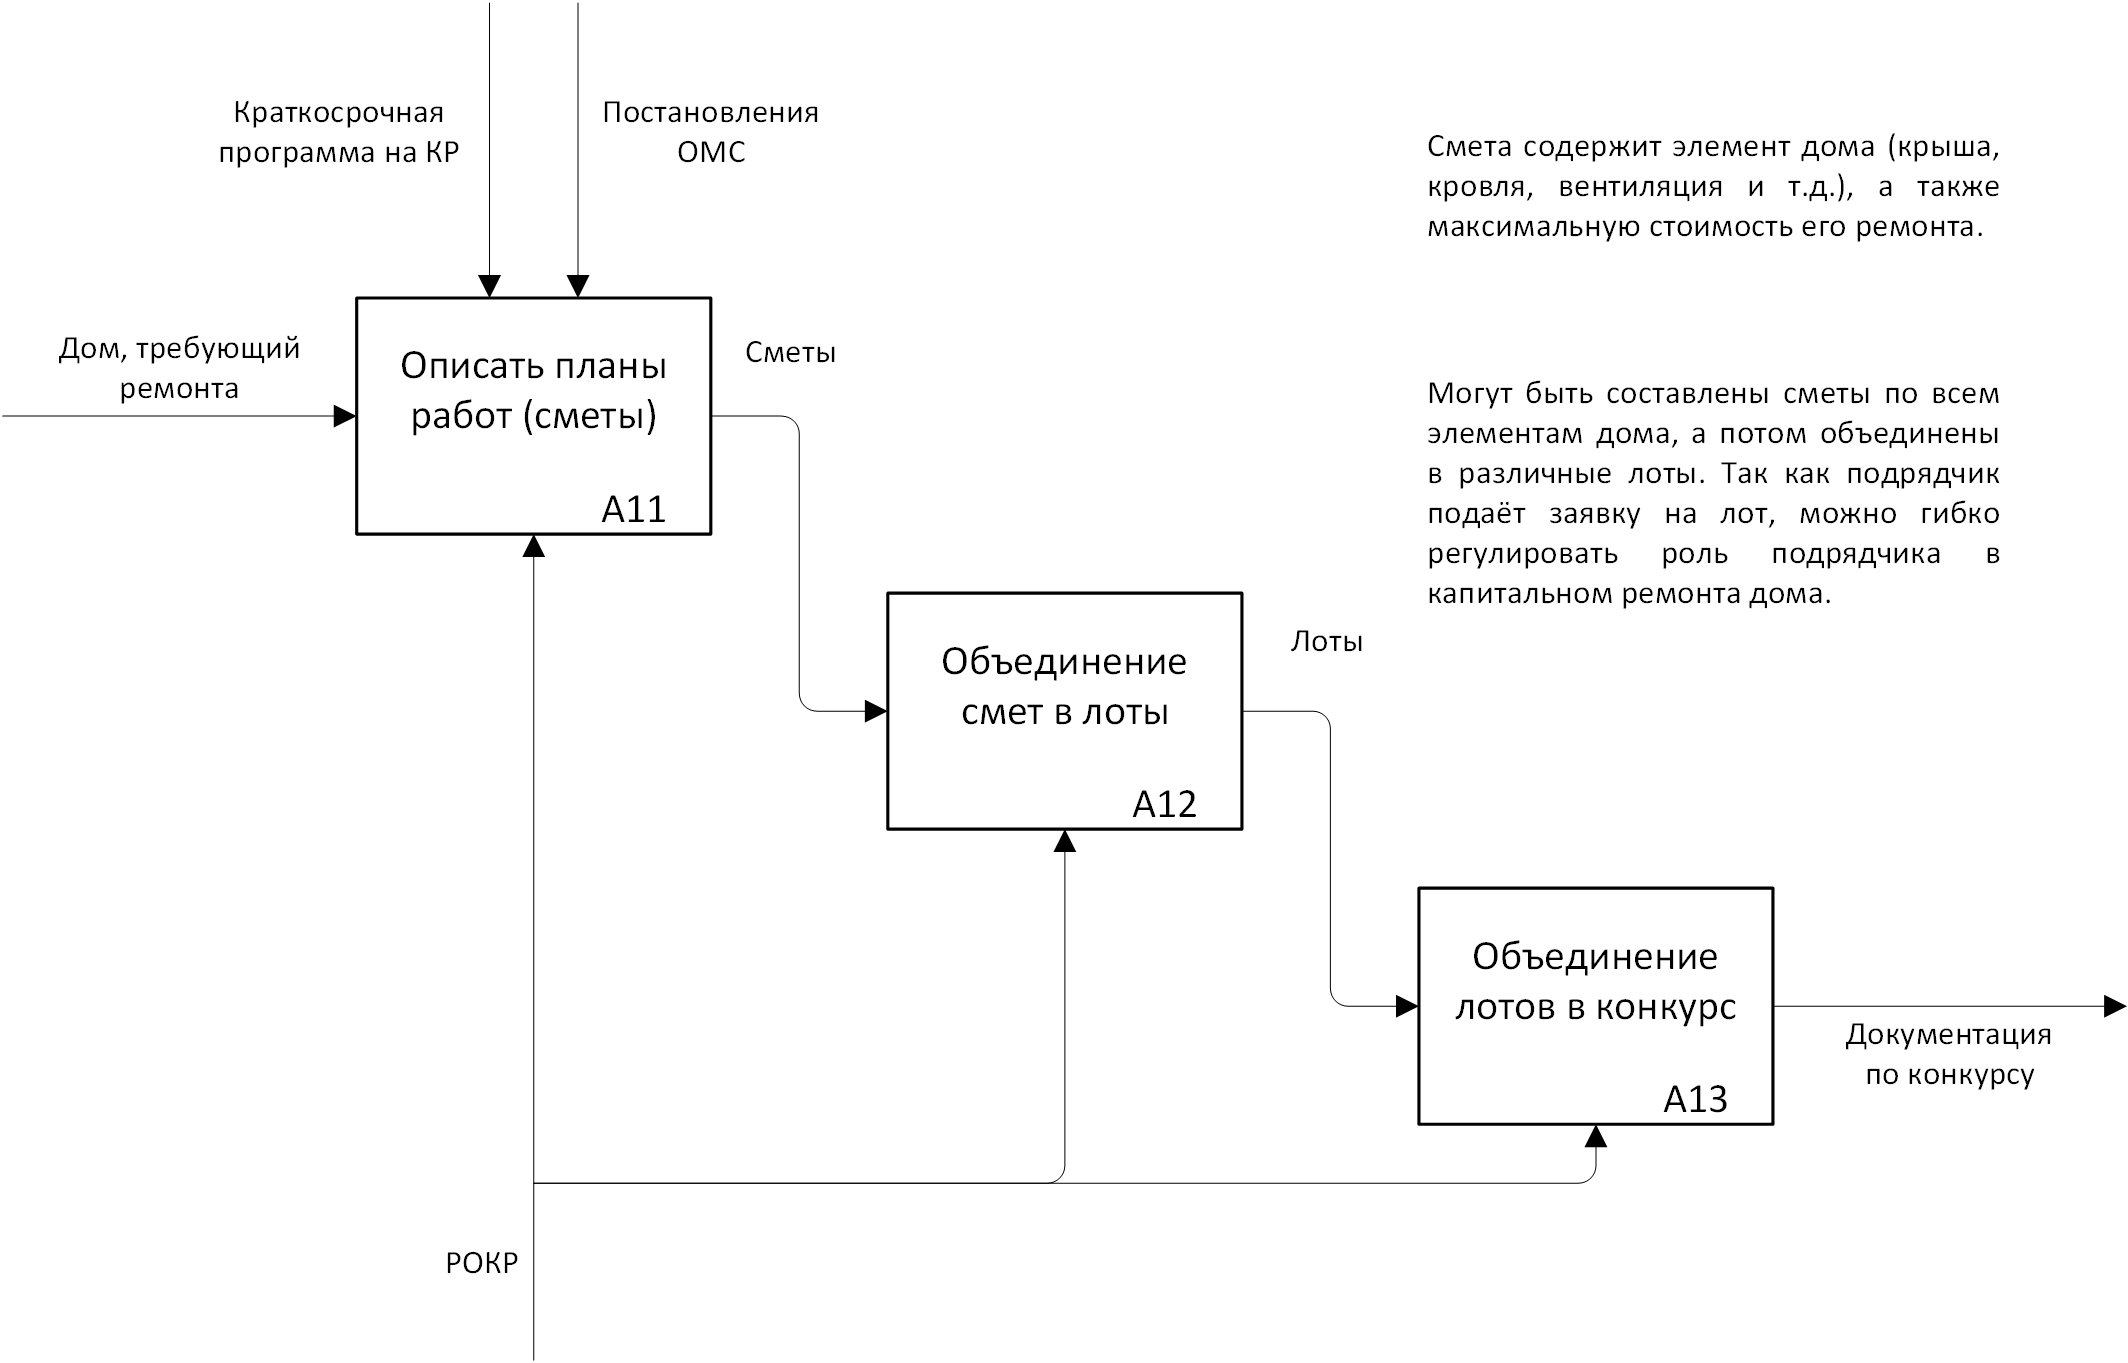
\includegraphics[width=\linewidth]{images/source-A1.png}
			\caption{Декомпозиция процесса <<Формирование конкурсов>>}
			\label{img:source-A1}
		\end{minipage}
		\hfill
	\end{center}
\end{figure}

Из схемы видно, что для формирования конкурса сперва следует сформировать сметы на выполнение работ по капитальному ремонту.
Некоторые заказчики называют данные документы планами работ, поэтому данное название также представлено на схеме.
Затем сметы объединяются в лоты, которые объединяются в конкурсы.
Все действия выполняет региональный оператор капитального ремонта.
По окончании этапа формирования конкурсов поступает документация по конкурсам, которая будет использована в дальнейшем.

За этапом формирования конкурса на проведение капитального ремонта следует этап проведение данного конкурса.

Декомпозиция проведения конкурсов представлена на рисунке~\ref{img:source-A2}.

\begin{figure}[h!]
	\begin{center}
		\begin{minipage}[h]{\linewidth}
			\centering
			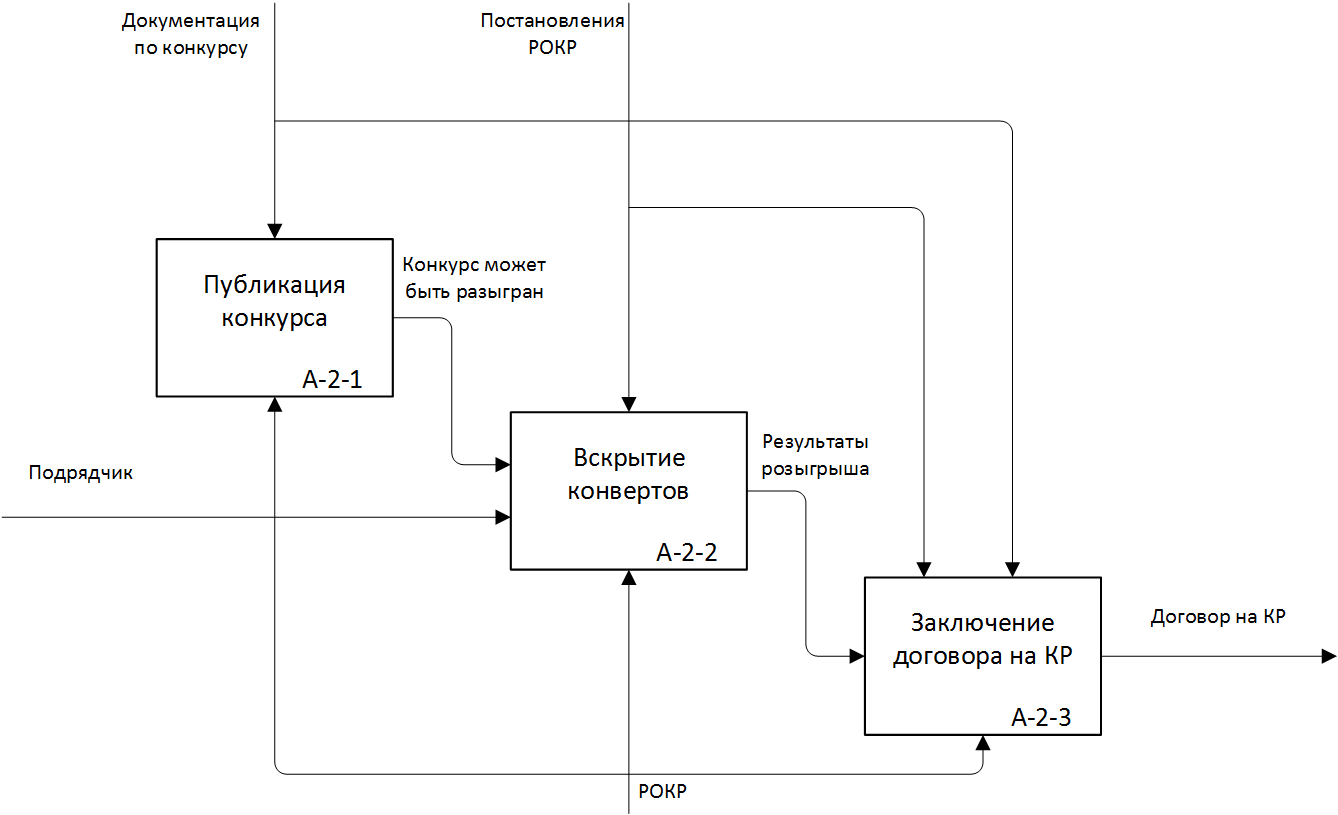
\includegraphics[width=\linewidth]{images/source-A2.png}
			\caption{Декомпозиция процесса <<Проведение конкурса>>}
			\label{img:source-A2}
		\end{minipage}
		\hfill
	\end{center}
\end{figure}

При проведении конкурса первым этапом следует публикация конкурса в средствах массовой информации.
Это сделано для того, чтобы подрядчики могли ознакомиться с требуемыми работами, описываемыми в планах работ (сметах), прикреплённым к лотам.
Затем, когда настаёт определённый промежуток времени, вскрываются конверты с заявками подрядчиков, которые были предоставлены ими заранее.
После вскрытия конвертов заключается договор на капитальный ремонт с победителем розыгрыша.

После проведения конкурса следует капитальный ремонт и процессы, с ним связанные.

Декомпозиция проведения капитального ремонта представлена на рисунке~\ref{img:source-A3}.

\begin{figure}[h!]
	\begin{center}
		\begin{minipage}[h]{\linewidth}
			\centering
			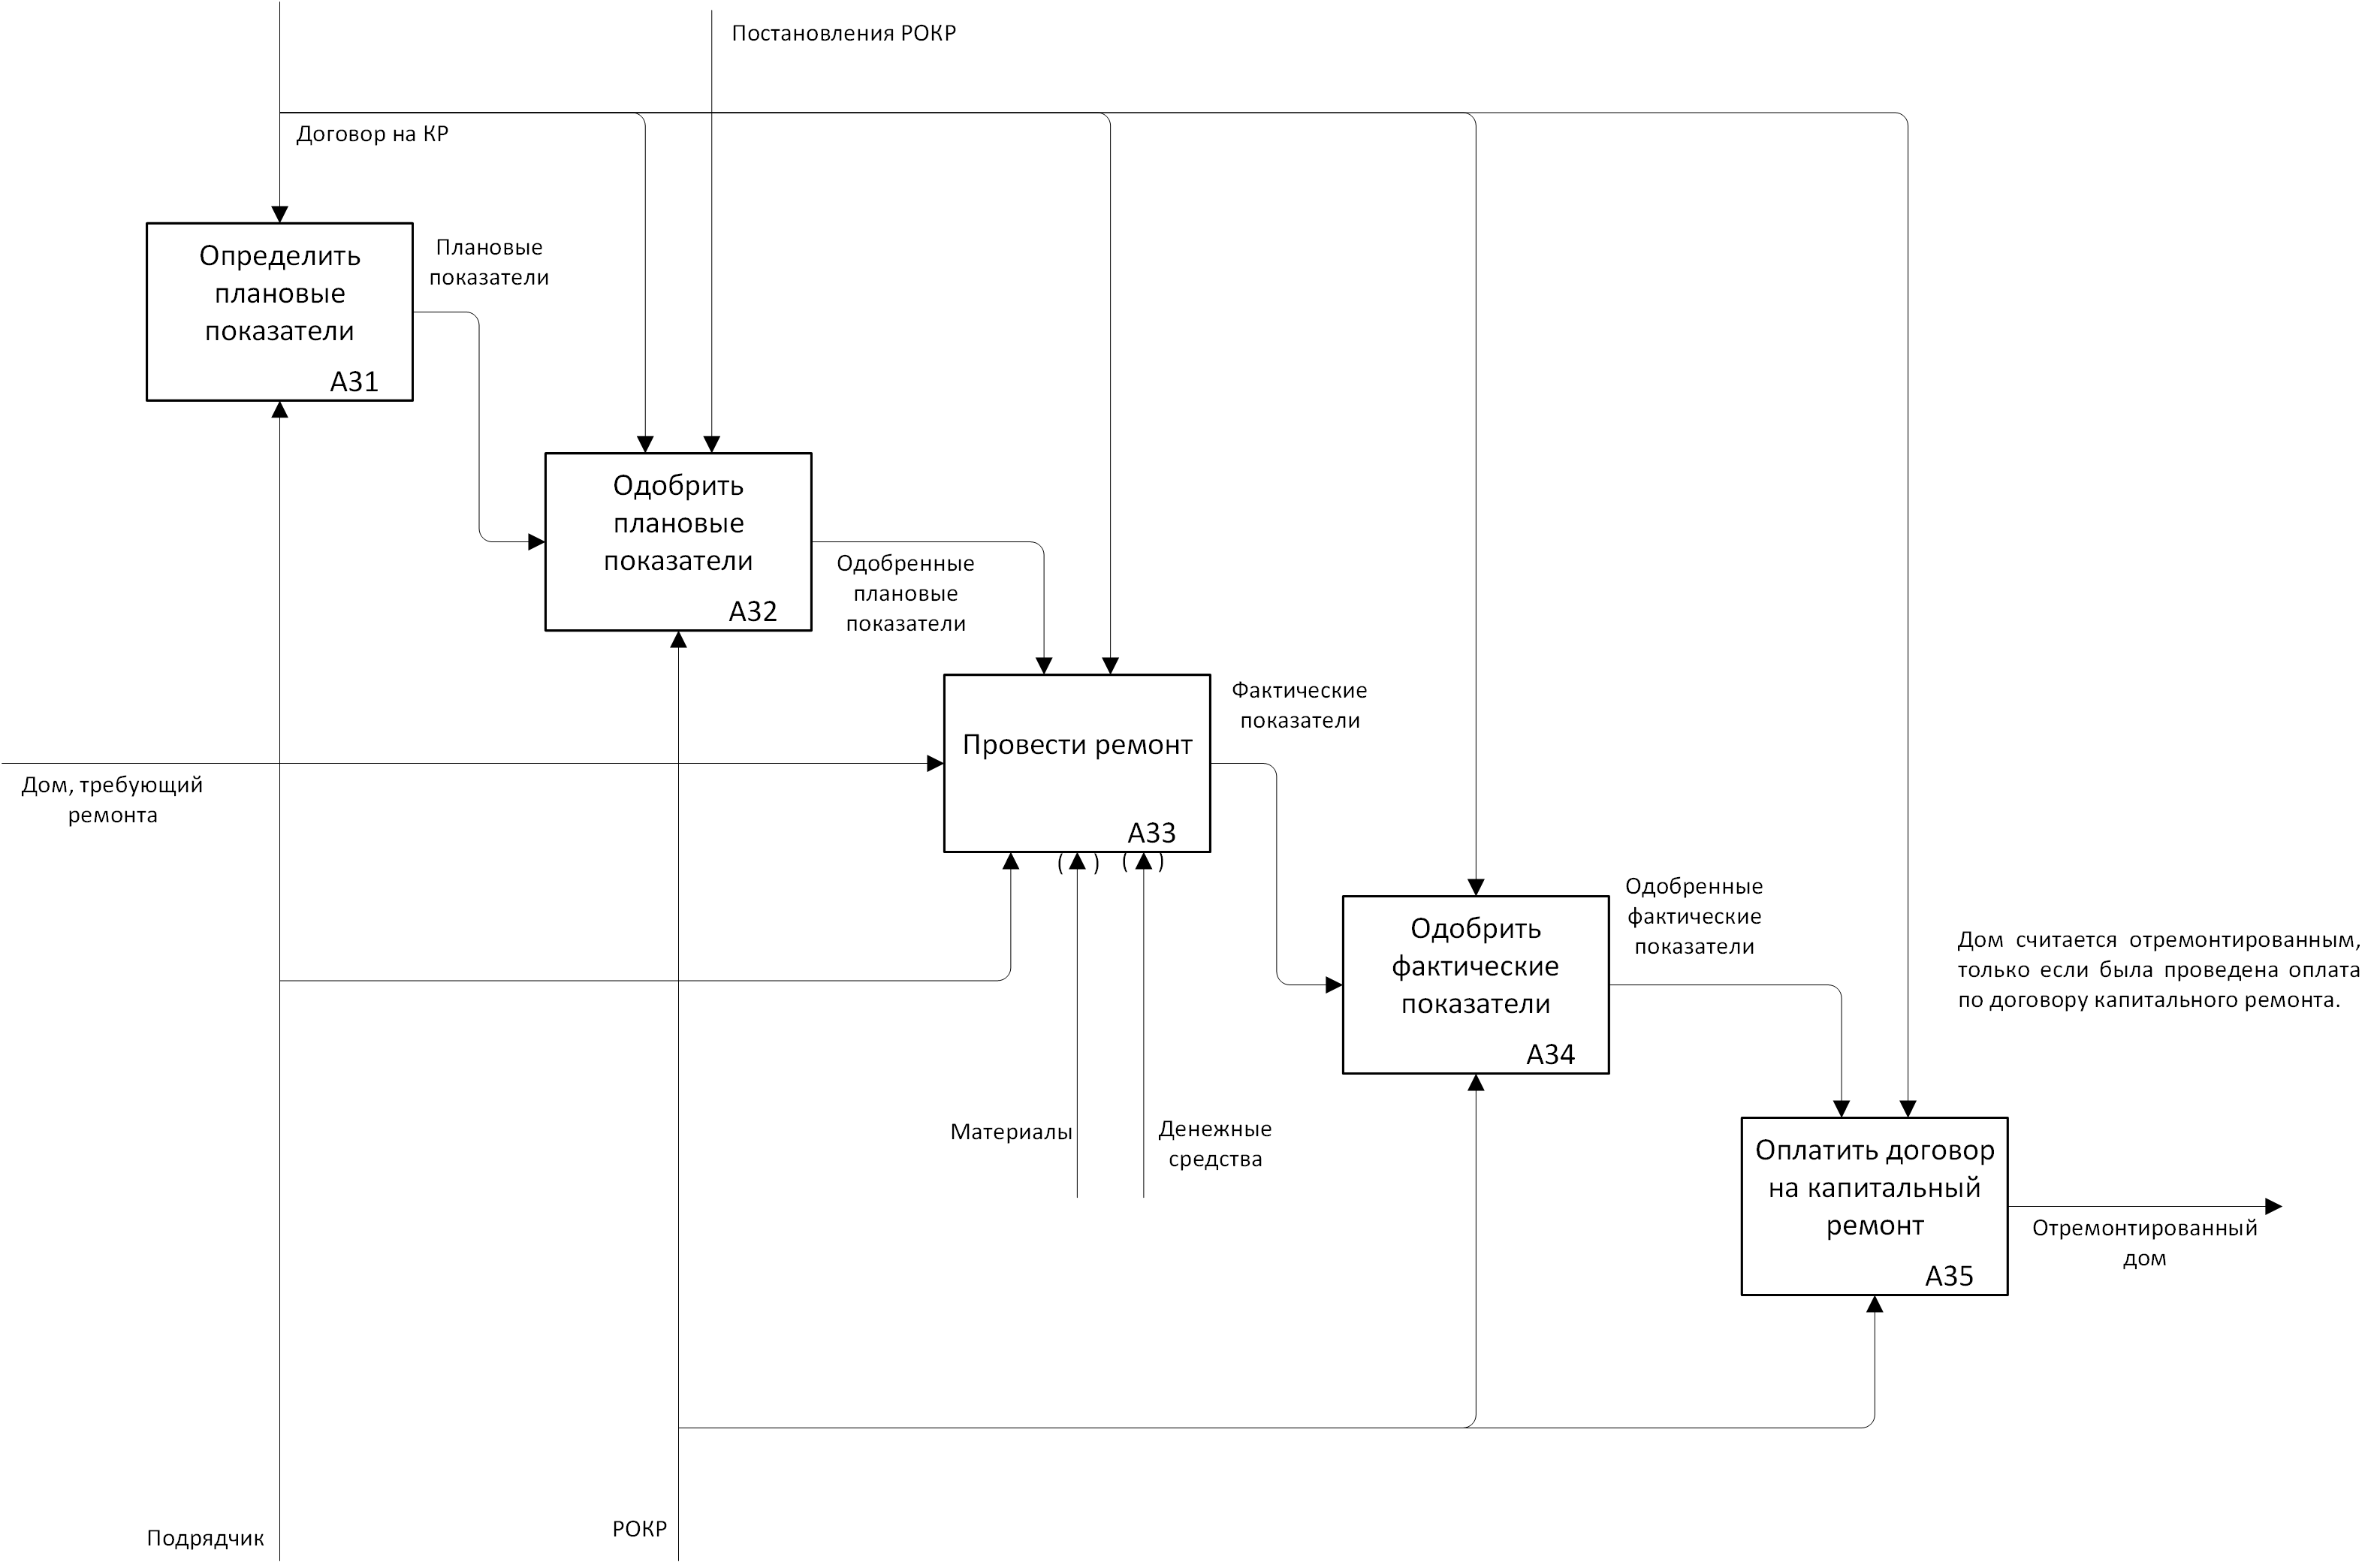
\includegraphics[width=\linewidth]{images/source-A3.png}
			\caption{Декомпозиция процесса <<Капитальный ремонт>>}
			\label{img:source-A3}
		\end{minipage}
		\hfill
	\end{center}
\end{figure}

При проведении основного процесса капитального ремонта сначала оцениваются плановые показатели по ремонту жилого фонда.
Это действие выполняется подрядной организацией.
Затем региональный оператор должен одобрить данные показатели.
После успешного одобрения подрядчиком производится непосредственно ремонт.
После ремонта возникают фактические показатели, которые следует одобрить.
Это действие выполняет региональный оператор капитального ремонта.
После того, как показатели будут одобрены, происходит оплата договора на капитальный ремонт.
На этом процесс проведения капитального ремонта считается завершённым.

\clearpage
\newpage